% ref: http://pgfplots.net/tikz/examples/bar-plot/
\begin{figure}[t]
\begin{minipage}[b]{1.0\linewidth}
    \raggedright
    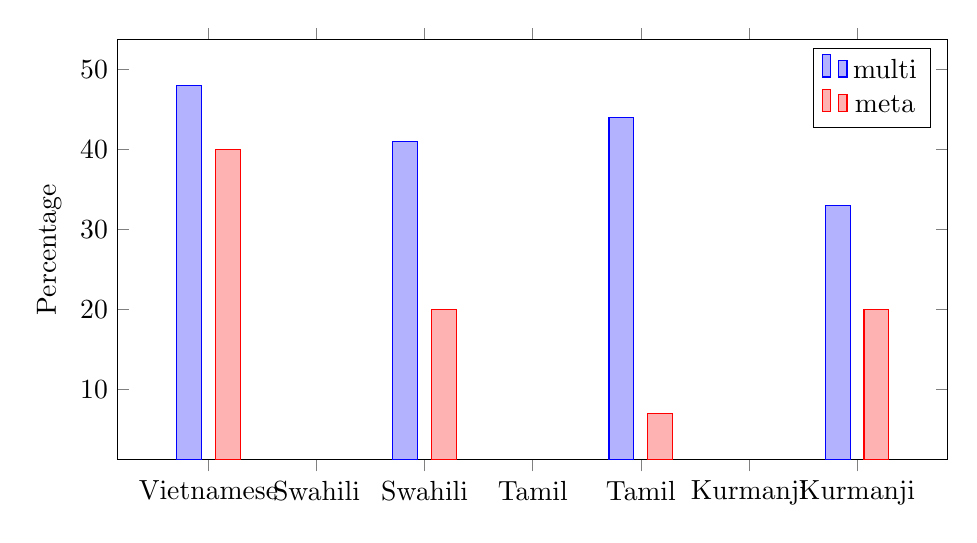
\begin{tikzpicture}
\begin{axis}[
	x tick label style={
		/pgf/number format/1000 sep=},
    ylabel= {Percentage},
	enlargelimits=0.14,
	symbolic x coords={Vietnamese,Swahili,Tamil,Kurmanji},
	xticklabel style={align=center},
	ybar=5pt,
	height=.57\textwidth,
	width=\textwidth,
	bar width=9pt,
]

\addplot 
	coordinates {(Vietnamese,48) (Swahili,41)
		 (Tamil,44) (Kurmanji,33) };

\addplot 
	coordinates {(Vietnamese,40) (Swahili,20) 
		(Tamil,7) (Kurmanji,20) };

\legend{multi, meta}
\end{axis}
\end{tikzpicture}
    \caption{CER relative improvement from LLP to FLP}
    \label{fig:impact-on-size}
\end{minipage}

\end{figure}
